
\subsection{Ikeda's method: from strip theory to semi-empirical formulas}
\label{se:semi-empirical methods}
In a ship's early design stage when only limited information is available, such as the ship's principal dimensions and the basic hull geometry, model test cannot be used. Therefore, several semi-empirical methods were proposed in the late 70th. The most recognize method was developed in a series of research articles \parencite{ikeda_roll_1978,ikeda_eddy_1978,ikeda_roll_1979,ikeda_components_1978,ikeda_velocity_1979}, often refered to as the Ikeda's method. This method divides the roll damping into five damping components, i.e., the friction component $B_F$, the eddy component $B_E$, the lift component $B_L$, the wave component $B_W$ and the bilge keel component $B_{BK}$, as in the following Eq.(\ref{eq:ikeda}), 

\begin{equation} \label{eq:ikeda}
B = B_F + B_E + B_L + B_W + B_{BK}
\end{equation}

where the wave and eddy components require strip theory based hydrodynamic analysis to get the ship's shape coefficients. The hydrodynamic analysis requires to get a ship's exact hull geometries. It might be time consuming to build the geometry model and perform the strip theory based hydrodynamic analysis. Sometimes, a ship's hull geometry is simply not available for such purposes. 

A simplified Ikeda's method was proposed by \parencite{kawahara_simple_2011} and is instead used in this study to calculate all the damping components including the eddy component $B_E$ and wave component $B_W$. The semi-empirical formulas describe four of the five roll damping components at motion frequency $\omega$ for a given roll amplitude $\phi_a$ at zero ship speed. A speed dependency was introduced by adding a fifth damping term $B_L$ and a speed correction to $B_W$ as described in \parencite{ikeda_velocity_1979} giving a function: 

\begin{equation} \label{eq:simplified_ikeda_equation}
\left( B_{44}, \  B_{F}, \  B_{W}, \  B_{E}, \  B_{BK}, \  B_{L}\right) = \operatorname{Ikeda_{simplified}}\left(L_{pp},beam,C_{b},A_{0},OG,\phi_{a},BK_{L},BK_{B},\omega,T,V\right)
\end{equation}

\parencite{kawahara_simple_2011} also prescribe the following limits to this method:
\begin{equation}
    \label{eq:SI_limits}
    \begin{align}
    0.5 \leq C_b \leq 0.85, 
    2.5\leq beam/T \leq 4.5,
    -1.5 \leq OG/T \leq 0.2, 
    0.9 \leq A_0 \leq 0.99, \\ 
    0.01 \leq BK_B/beam \leq 0.06,
    0.05 \leq NK_L/L_{PP} \leq 0.4,
    0 \leq \hat{\omega} \leq 1.0
    \end{align}
\end{equation}

The detailed formulas within $f$ can be referred to \parencite{kawahara_simple_2011}, \parencite{ikeda_velocity_1979} and the actual implementation \parencite{alexandersson_martinlarsalbertrolldecay-estimators_2020}.

%The Simplified Ikeda method \cite{kawahara_simple_2011} has been implemented \cite{alexandersson_martinlarsalbertrolldecay-estimators_2020} with the intention to be used both as a benchmark and maybe also as a sub-component of a new method. The examples from \cite{kawahara_simple_2011} was recalculated to check that the method has been implemented correctly. The authors have been unable to find other ways to validate the implementation, which introduces some uncertainty to the comparisons. The method has been implemented as a function where the total roll damping and its component is calcultated: 


%The Ikeda method has been used to calculate the roll damping for the RoRo vessel Faust \parencite{soder_assessment_2019}. As an example, Fig. \ref{fig:ikeda_vs_simplified} shows a comparison between roll damping components calculated with the original \emph{Ikeda's method} based on strip theory calculation and the simplified Ikeda's method. The roll damping is under-predicted with the simplified method for this particular case which is expected according to the limitations of this method  \parencite{kawahara_simple_2011}.

%\begin{figure}[H]
%    \centering
%    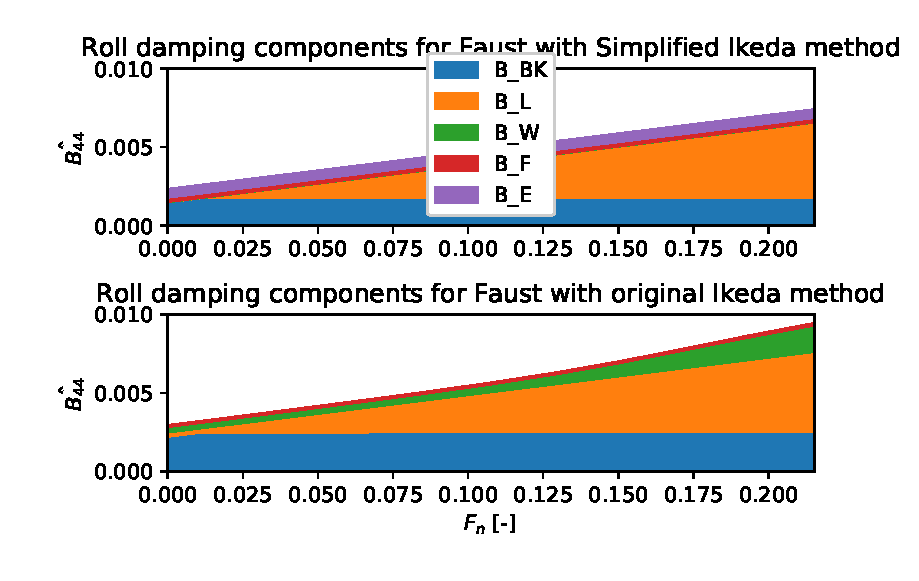
\includegraphics{figures/ikeda_vs_simplified.eps}
%    \caption{Roll damping components calculated with Ikeda and Simplified Ikeda %for PCTC Faust}
%    \label{fig:ikeda_vs_simplified}
%\end{figure}


